%%%%%%%%%%%%%%%%%%%%%%%%%%%%%%%%%%%%%%%%%%%%%%%%%%%%%%%%%%%%%%%%%%%%%%%%%%%%%%%%
% Author : Radek Zobaník, Tomas Polasek (template)
% Description : Seventh exercise in the Introduction to Game Development course.
%   It deals with the creation of a Game Design Document, presenting a short 
%   pitch for a potential game project.
%%%%%%%%%%%%%%%%%%%%%%%%%%%%%%%%%%%%%%%%%%%%%%%%%%%%%%%%%%%%%%%%%%%%%%%%%%%%%%%%

\documentclass[a4paper,10pt,english]{article}

\usepackage[left=2.50cm,right=2.50cm,top=1.50cm,bottom=2.50cm]{geometry}
\usepackage[utf8]{inputenc}

% Hyper-Text References
\usepackage{hyperref}
\hypersetup{colorlinks=true, urlcolor=blue}

% Drawing Images and Graphs
\usepackage{tikz}
\usepackage{pgfplots}

% Page Utilities
\usepackage{graphicx}

% Image Sub-Captions
\usepackage{subcaption}

\newcommand{\ph}[1]{\textit{[#1]}}

\title{%
Game Pitch Document%
}
\author{%
[Name] [Surname] ([Login])%
}
\date{}

\begin{document}

\maketitle
\thispagestyle{empty}

{%
\large

\begin{itemize}

\item[] \textbf{Title:} \ph{On the Edge}

\item[] \textbf{Genre:} \ph{Adventure, Horror, puzzle}

\item[] \textbf{Style:} \ph{3D, semirealistic}

\item[] \textbf{Platform:} \ph{Pc, PS5}

\item[] \textbf{Market:} \ph{Horror game players}

\item[] \textbf{Elevator Pitch:} \ph{Solving a mystery with many possible outcomes under the constant dread}

\end{itemize}

}

\section*{\centering The Pitch}

\subsection*{Introduction}
You are solving a mystery like a real detective with all the clues collecting and assumptions making, all of that while running away and hiding from an unknown threat.


\subsection*{Background}

I really enjoyed the core idea of Sherlock Holmes: Crimes and punishment, the way you collect clues and use the gained knowledge to try to solve what really happened. This was my first inspiration. But my biggest problem with that game was, that it was basically a walking simulator. There were some puzzles that were not challenging but fun anyway, but that was it. There was no drama, there was no time pressure. And the final conclusion of every case was kinda obvious. It was not really challenging. So i want to change that.\newline

Detective books. How there are always many possible outcomes of what really happened and you try to guess it. And how with more and more informations you get closer and closer to knowing what really happened.\newline

I really like horror games for their constant feeling of danger. This game should have kinda same atmosphere as Amnesia games (my favourite Amnesia: Rebirth). The little cracks and sounds from the distance, like someone or something is near you and is always watching you. That would solve the stale atmosphere of the "walking-only" detective genre. 


\subsection*{Setting}
This is a narrative driven game, where you follow a story of a young woman who is trying to find what happened to her sister. Player will follow a core linear story, but his gameplay will hugely alter the situations. It will be up to player to decide which place to search first and which clue to follow. In the end the player can miss some parts.\newline

The main part of the game takes place in a small village in a mountains. That is the place where her sister lives(lived). A lot of wooden buildings and structures, based in today's world.\newline

Some parts will take place in main character's imagination or in her childhood memories.


\subsection*{Features}

\begin{itemize}
    \item Challenging puzzles
    \item Decisions altering gameplay and ending
    \item Collecting clues while having the freedom of what to do next
    \item Scary atmosphere
    \item Stealth action 
    \item Nerve wracking chase sequences
\end{itemize}


\subsection*{Genre}
It will be a combination of a horror game and a detective adventure. Your task is to survive, but at the same time to solve the mystery by collecting clues and using your deduction to decide what to do next. Player will have to hide and run away with very little means of protection.

\subsection*{Platform}
It will be released on PC and and Playstation (on their newest released console)

\subsection*{Style}
Game would look like something like these pictures(taken from games Life is Strange 2 and What remains of Edith Finch). But the world will be much darker with higher contrast of light vs darkness. Places without any danger will be more colourful and lighter (imaginations will be especially colourful).

\begin{figure}[h]

\centering

\begin{subfigure}{0.29\linewidth}
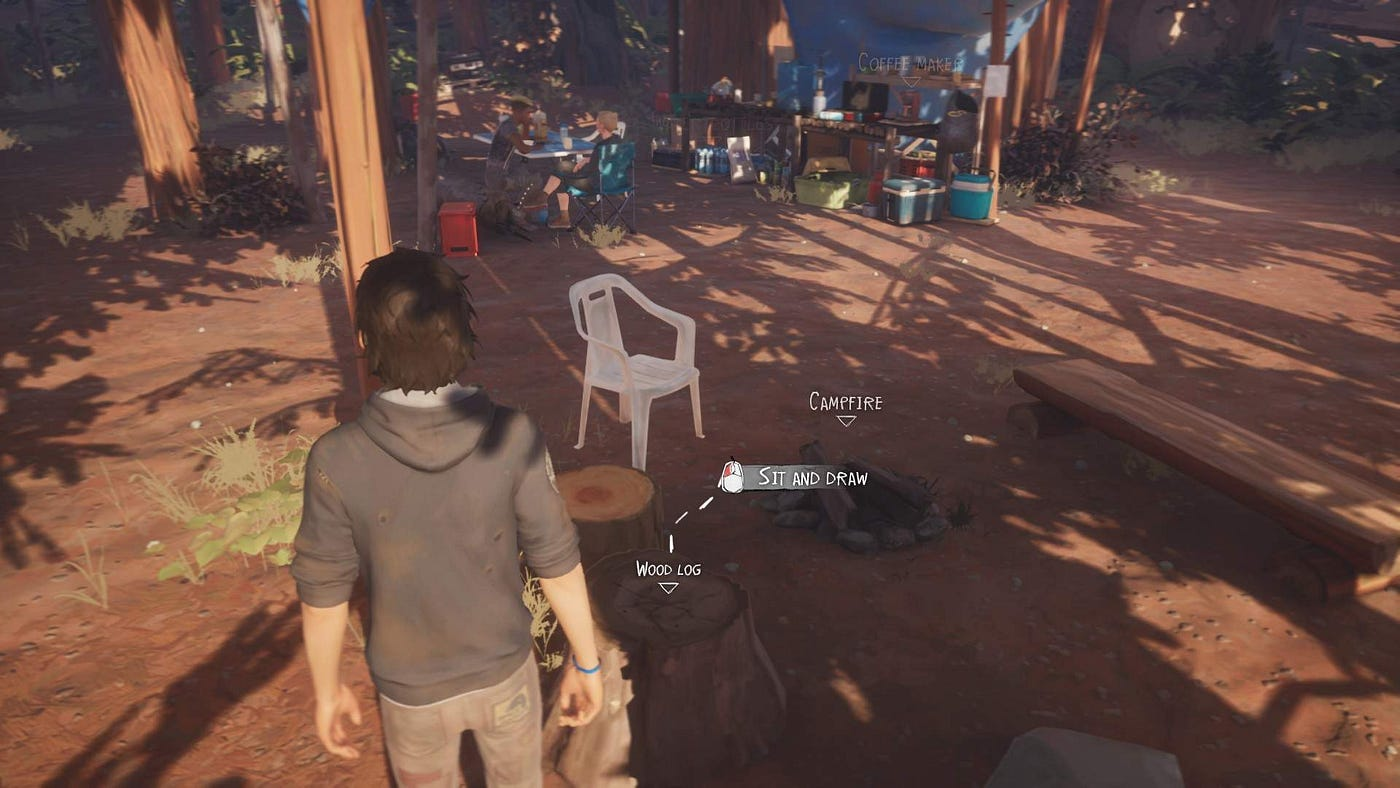
\includegraphics[width=\linewidth]{img1.jpg}
\captionof{figure}{Forest scene 1}
\label{Fig:Style1A}
\end{subfigure}\hfill
%
\begin{subfigure}{0.29\linewidth}
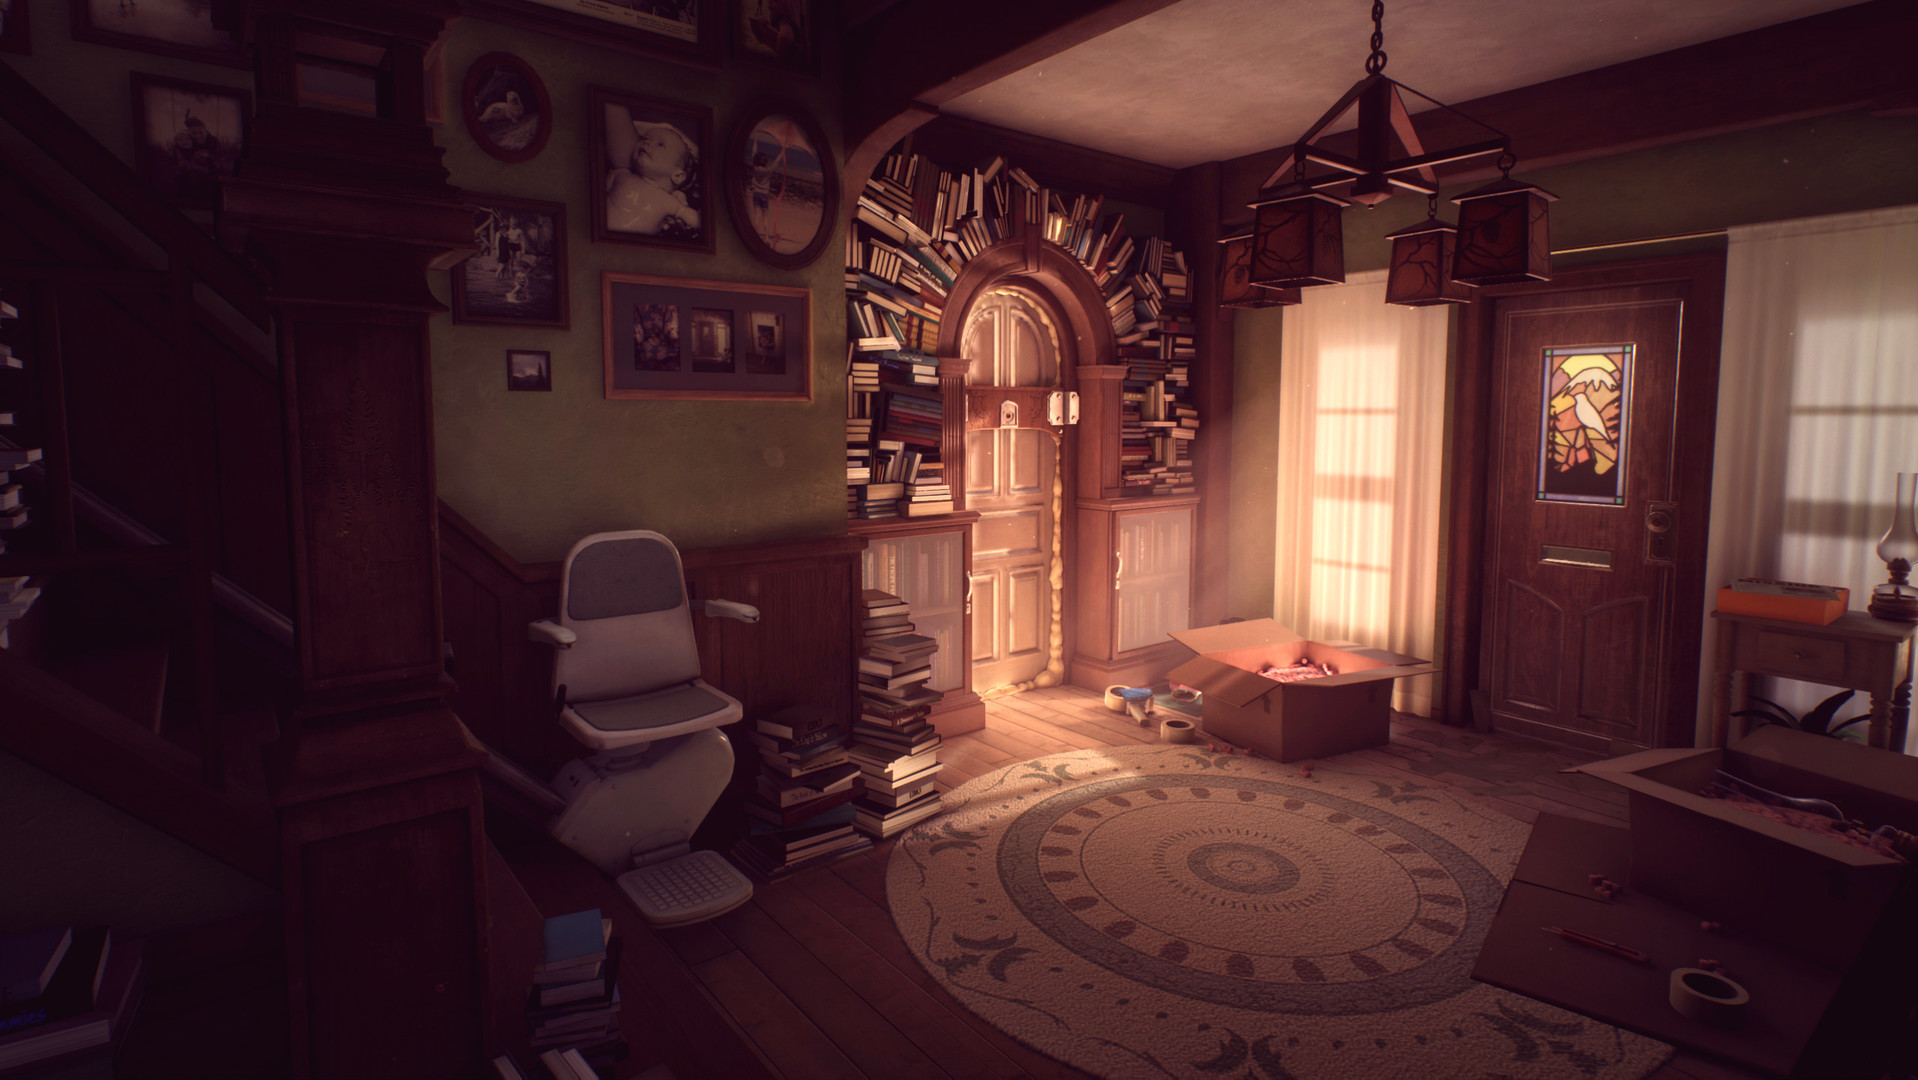
\includegraphics[width=\linewidth]{img2.jpg}
\captionof{figure}{Interior scene 1 }
\label{Fig:Style1B}
\end{subfigure}\hfill
%
\begin{subfigure}{0.29\linewidth}
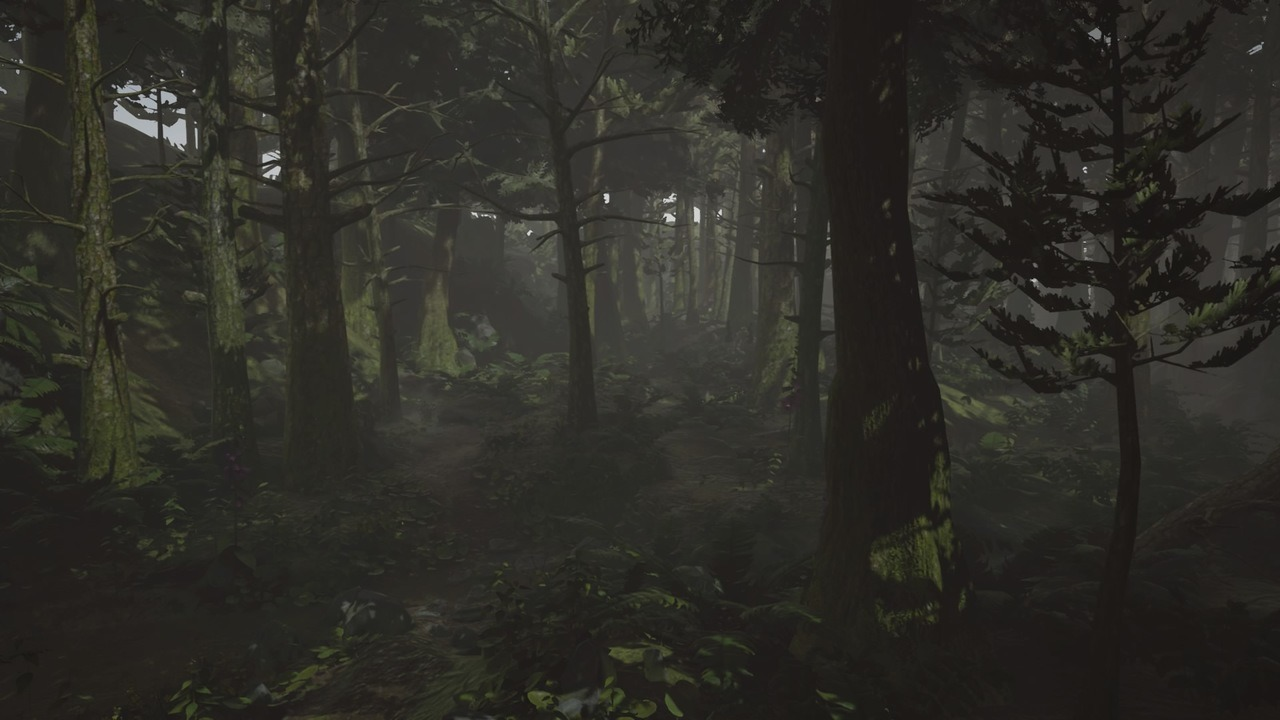
\includegraphics[width=\linewidth]{img3.jpg}
\captionof{figure}{Forest scene 2}
\label{Fig:Style1C}
\end{subfigure}

\end{figure}

This is the first concept of the main location. Small village in the forest. Building situated around one main road. Active quarry at the end of the road.
\begin{figure}[h]
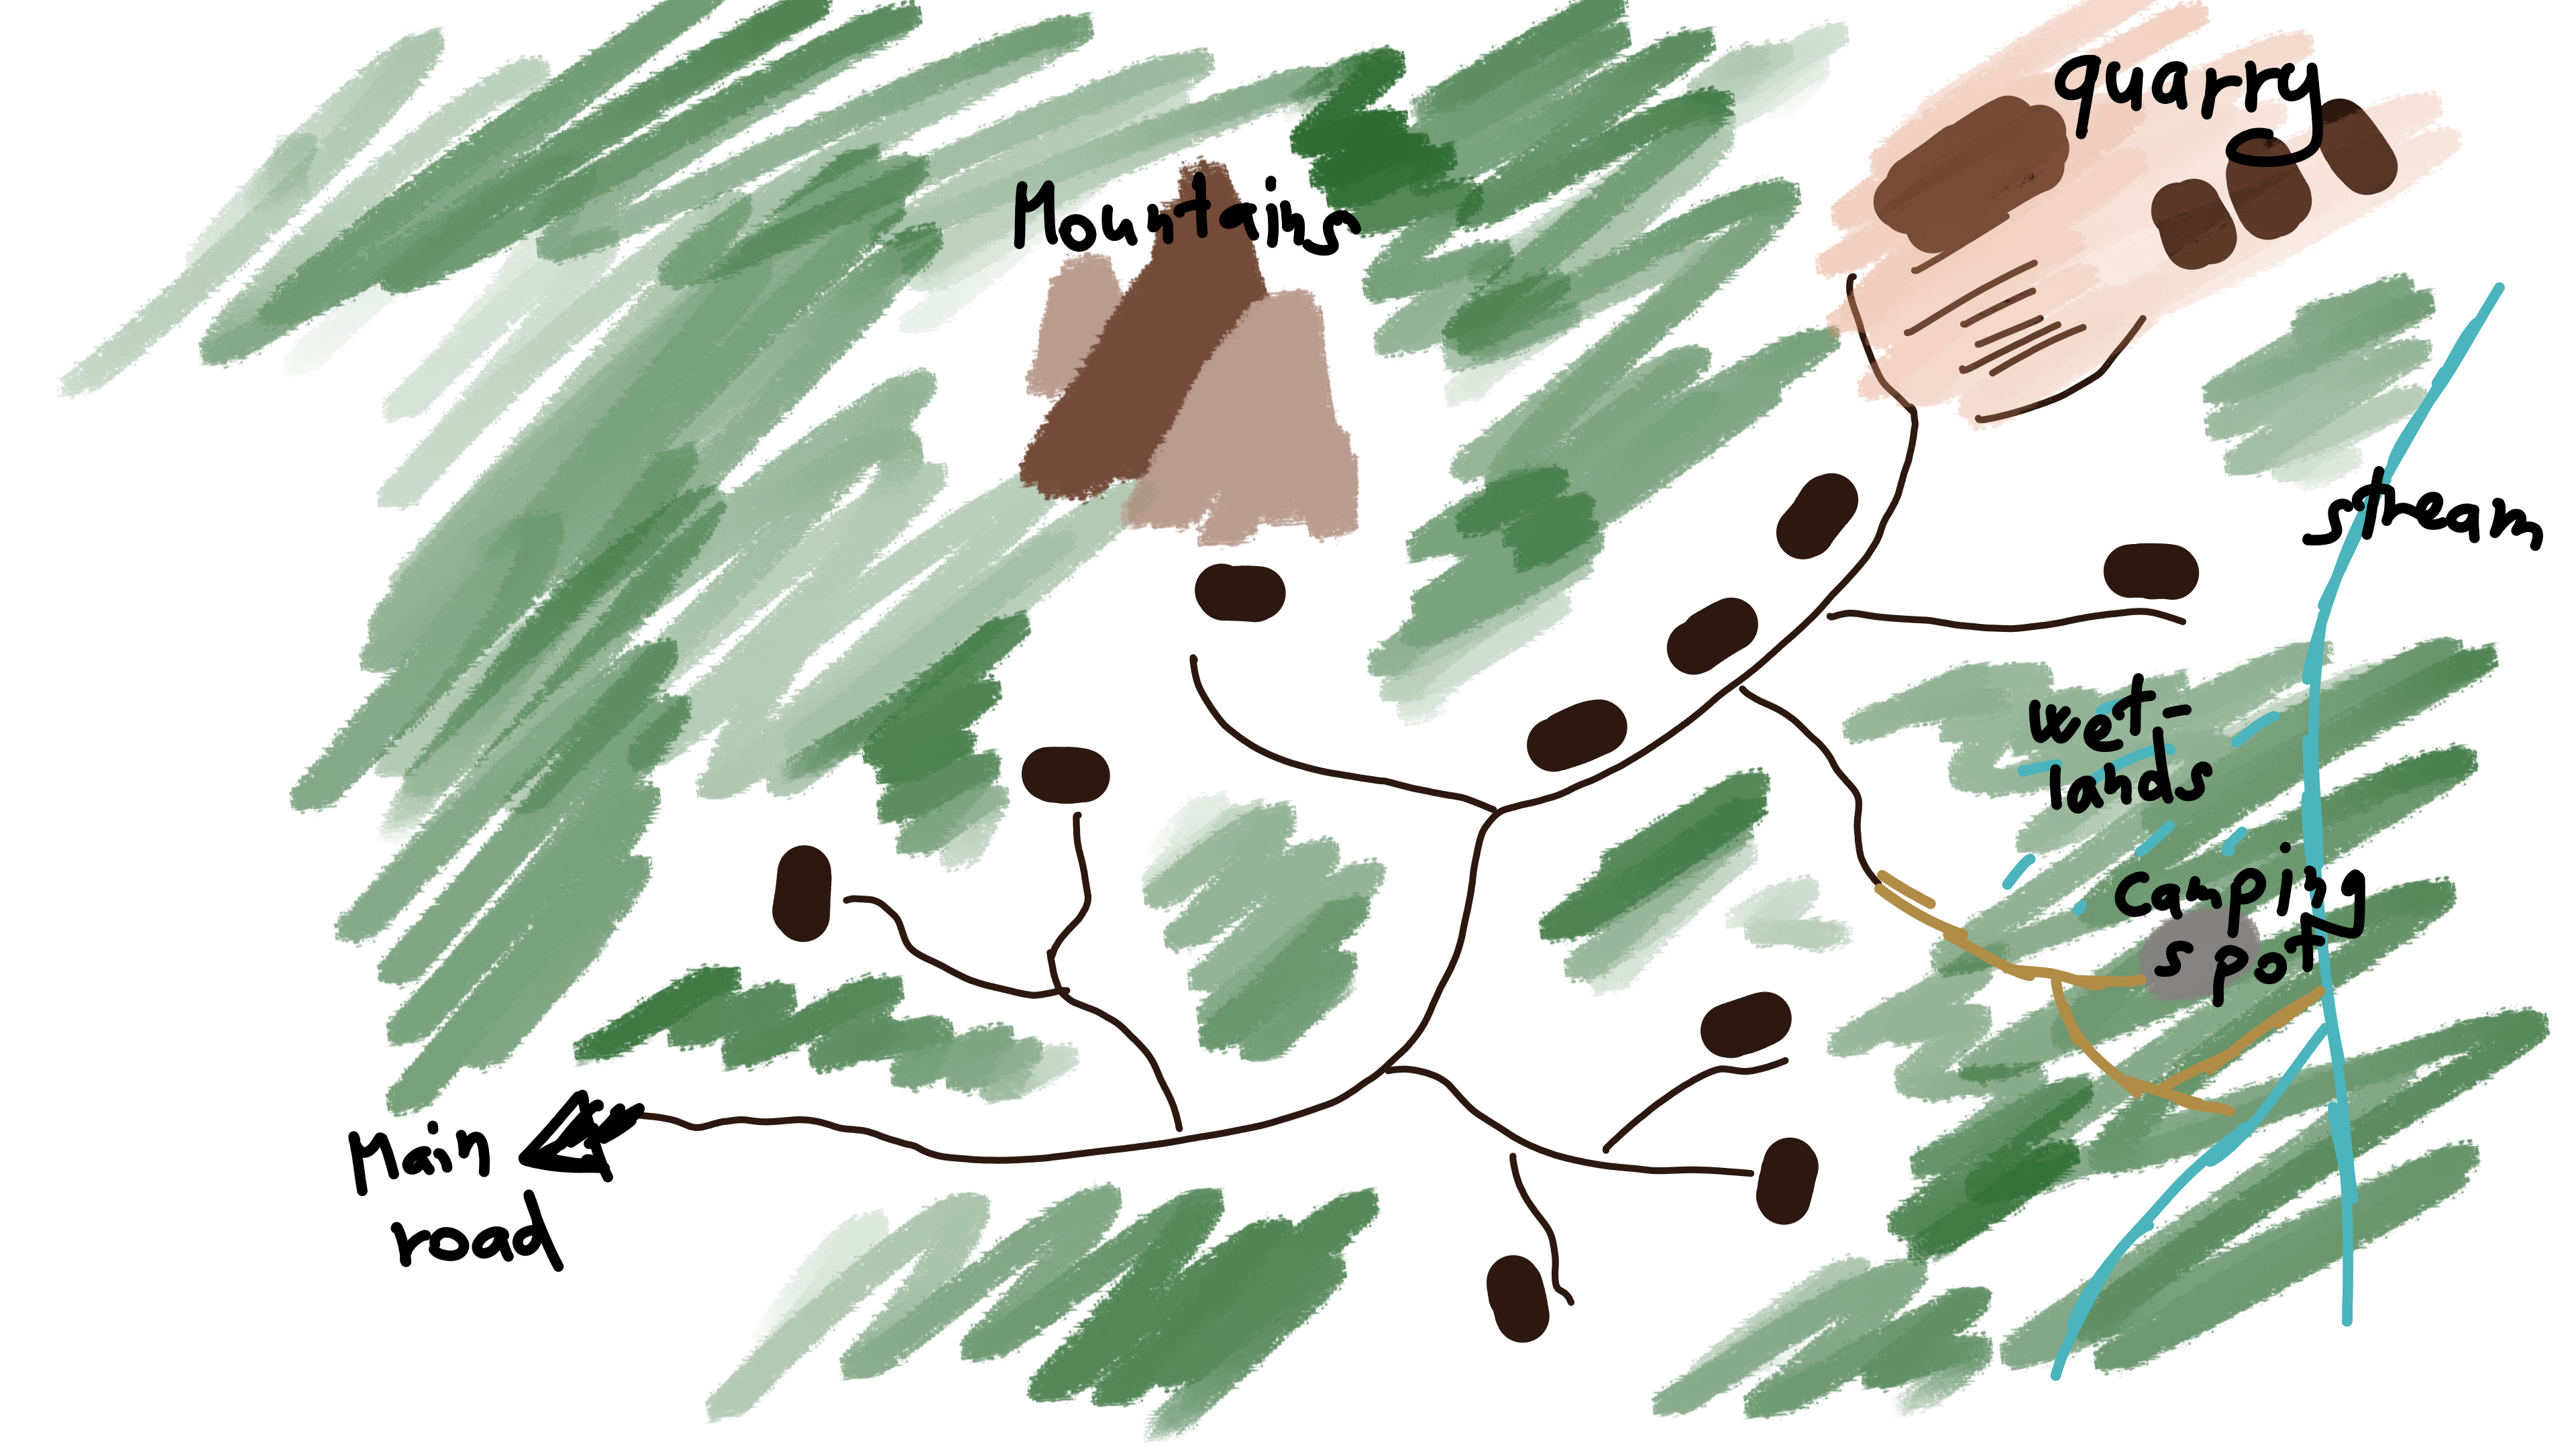
\includegraphics[width=18cm, height=11cm]{Map.png}
\end{figure}
\end{document}
